\chapter{Easy Web Content Site Builder}

The Easy Web Content Site Builder, also called EWS, is the main project we are working. This project intends to complete the existing Easy Web Content service by enabling the user to create a new website from scratch.
%descriptopn of EWS
Basically The site builder will make extensive usage of Ajax\footnote{Asynchronous Javascript and XML}. The main directions of the project are
\begin{itemize*}
\item Be the most simple in terms of user experience
\item Propose simple to create but adapted styles and easy to customise
\item Do not have the drawbacks of the competitors
\item Have the advantages of the competitors
\item Be scalable
\item Be secure
\item Target users : 2/3 of them have no HTML/CSS knowledge
\end{itemize*}
%show a sample of the concurrence

The major competitors(See Appendix \ref{annexe:ews-competitors})  in the market of site builders are Weebly, Drupalgardens, Basekit and Squarespace.
Weebly and BaseKit use a drag and drop approach instead of Drupalgardens and Squarespace which is more a blog-like content management system.

So the first step into the project was to brainstorm about the feasibility of the software. We did several research of what was already existing in the market. Writing down the strengths and weaknesses of the most famous site builders. At the same time we specified the structure of the information system which would allow the site builder to be scalable, and modular. We try to figure what was the best choices between architecture and programming languages. After a week we decided to adopt PHP MySQL and Javascript instead of J2EE , GWT. 

The developers into the team are more familiar with these technologies. So we designed a relational model for the MySQL database(\ref{figure:ews_rev_eng_dec} p.\pageref{figure:ews_rev_eng_dec}) that matched our first expectations in term of page creation and page organisation.
\begin{figure}[h!]
\centering
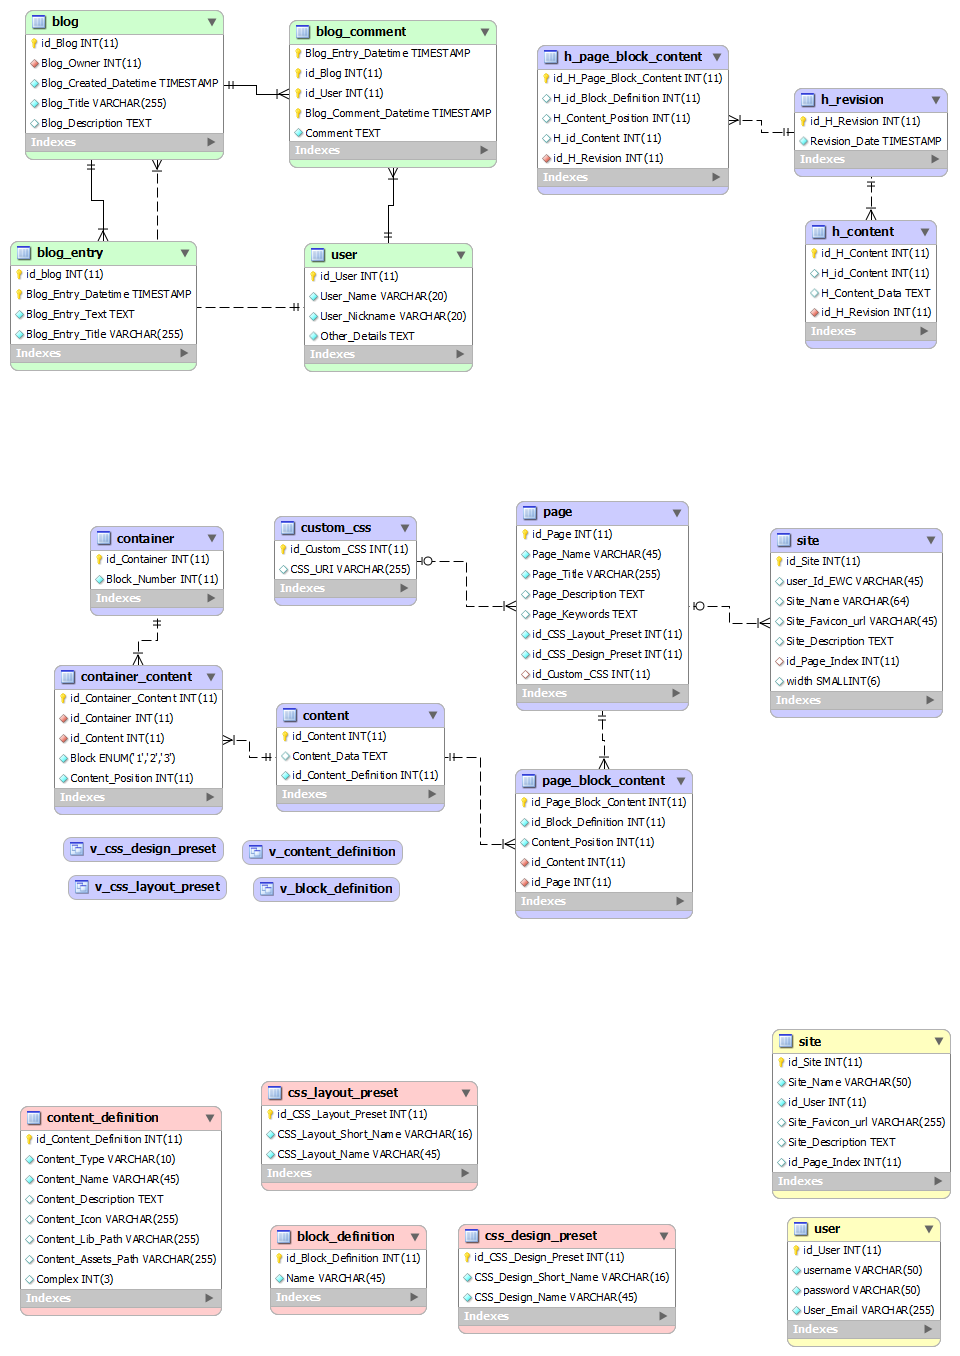
\includegraphics[width=.55\textwidth]{img/reverse_eng_15-dec-2010.png}
\caption{MySQL Database architecture }
\label{figure:ews_rev_eng_dec}
\end{figure}
We also had to design the overall architecture of the server (cf. figure \ref{figure:ews_archi_before} p.\pageref{figure:ews_archi_before}). Then, in order to scale the application to cloud computing, we made changes to the architecture(cf. figure \ref{figure:ews_archi_after} p.\pageref{figure:ews_archi_after}).


\begin{figure}[h!]
\centering
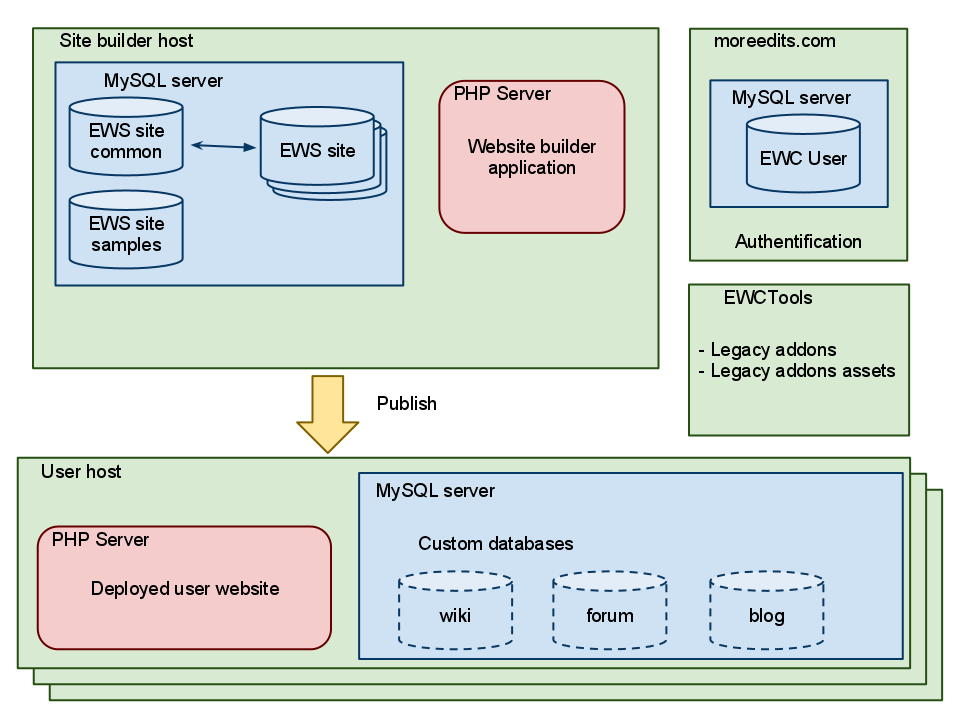
\includegraphics[width=.55\textwidth]{img/ews_archi_before.png}
\caption{Basic EWS architecture }
\label{figure:ews_archi_before}
\end{figure}

\begin{figure}[h!]
\centering
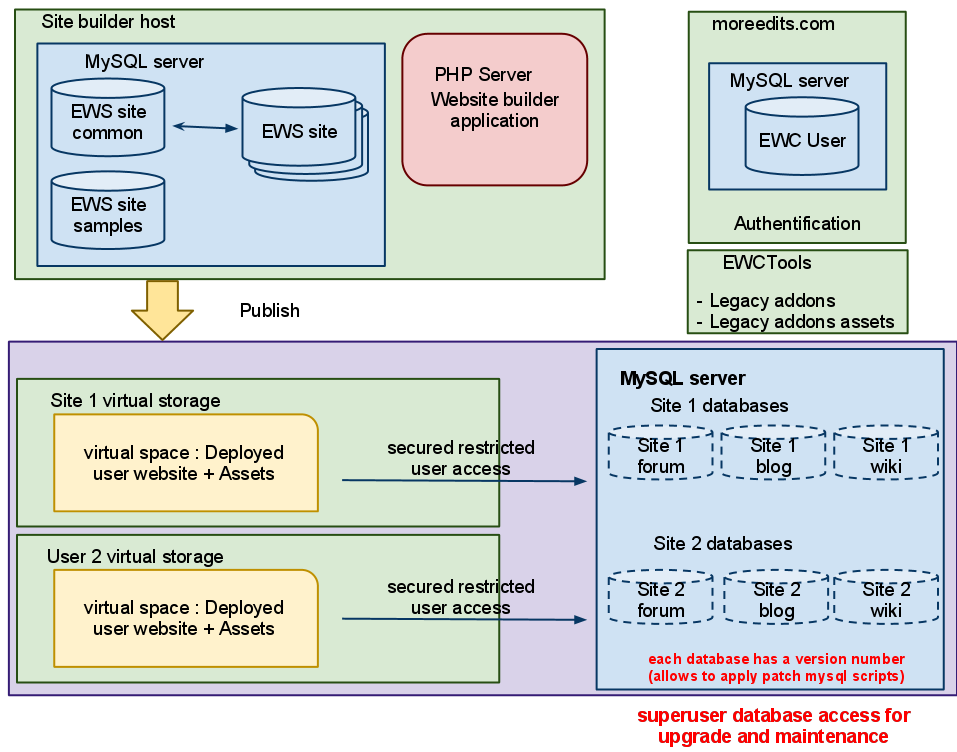
\includegraphics[width=.55\textwidth]{img/ews_archi_after.png}
\caption{Cloud optimiwed EWS architecture }
\label{figure:ews_archi_after}
\end{figure}

\begin{itemize*}
\item a database to store common data (data shared through the application)
\item a database to manage users and sites
\item one database per site 
\end{itemize*}

To allow better security, at the creation of a new site database the system creates a specific MySQL user for this database which have specific permissions only on that database. It can access common database data thru VIEWS.
% databases architecture illustration
After several meetings we decided to adopt a system that stores the informations of each pages created by the editor into a database. To allow less process time, the user will be able to publish his pages, which will result in the system creating plain php files containing all the information of the page.

\section{Framework}

To facilitate the development and maintainability of the application, we had to code using a Model View Controller pattern. The first thing that came to mind to adopt this pattern was to use a Php Framework. Many of them exist on the internet, for example Zend, Symphony, CakePhp, ... 

After looking at some of them, especially Zend, we figured out that using such a Framework would mean learning it. And it could be weeks before we were comfortable with it, let alone the fact that every six month new interns would come and would probably have to learn it too. The best solution for us considering the deadline we had on the project was to create our own MVC Framework. It took us less than a week to build the core features of this framework. Building our own framework has some advantages:
\begin{itemize*}
\item In a learning point of view, it is very interesting as it would help us understand some useful mechanism of Php
\item We would have total control over it and would be able to add features as we need them.
\end{itemize*}

The way our framework works is pretty simple. It redirect all request to one single entry point (index.php). This entry point would then call the appropriate controller and action. The controller then requests the database given the model we need and then call the appropriate view. This separates easily all 3 parts of the MVC pattern.
Also, the framework is object-based: 
\begin{itemize*}
\item Each Controller is a Php class that inherits the core controller class. It contains all the functionalities needed to handle a page request, to redirect a page, to get the data sent by the user, ...
\item Each Model is a Php class that inherits the core model class. It contains all the functionalities to access the database and request it.
\item Each view is a phtml file in which we print the content of the request.
\end{itemize*}

Developing an object-oriented application makes it way more scalable and reusable. It is the right way to develop a web application. During my 6 months at HindSite Interactive, I have worked on projects that had not been developed with object-oriented programming, and it was really hard to understand the code and be able to work efficiently with it. 

Later in the development of the application, we started adding features to the core of our framework. As an example, we created a special Controller, called AjaxController, that would be the type of controller to handle Ajax requests. Every other controller that would be called via Ajax would not process any treatment.

Another advantage of this framework is that the files are stored in different folders, so it is easier to localize the different elements. Most of the client projects I have worked on had all the files stored in one single folder, which can get really messy when this is a big project.
Here is the tree of the framework:
\begin{verbatim}
+---application
|   +---controllers
|   +---models
|   +---views
+---config
+---library
|   +---core
|   +---external
+---public
|   +---css
|   +---js
|   index.php
\end{verbatim}

\section{User Experience}


The main part of an application aimed at having people sign up for the services you provide is the user experience. If in the first few minutes of using the application the user feels lost or does not know how to perform the tasks he wants to, he is not going to sign up and will leave to the competitors. 

There are so many famous site builders in the Internet that we will surely not be the primary target of users. So when a user lands on our application, we need to keep him and have him sign up. So from the start of the development, we made a priority of providing the user with an easy interface, along with intuitive functionalities.
We had meetings once in a week to see which directions to take in terms of usability. Concerning the graphic user interface, the work was done by designers and we then had to convert their ideas to html and css code. The part that concerned us web developers was the intuitive functionalities. And in web language, this means programming in JavaScript / AJAX.

\subsection{JavaScript}

JavaScript is a client side programming language. It is interpreted by the user's web browser and runs on his computer, with no connection to the server whatsoever. When a web page is served to the user, JavaScript enables to extend the user experience. Some of the interesting functionalities of JavaScript are:
\begin{itemize*}
\item Binding events to the mouse or keyboard of the user
\item Changing the way a page look (modifying the css of an element)
\item Handing the DOM (Document Object Model) which means Create, Read, Update or Delete the html content of the page.
\end{itemize*}

Here are example on how you can achieve these features :
\lstset{language=Javascript}
\begin{lstlisting}[label=javascript_event,caption=Binding an event in Javascript]
window.onclick = function(){
	// code here
}
\end{lstlisting}
\begin{lstlisting}[label=javascript_appearance,caption=Modifying the css of an element ]
document.getElementById("anElement").style.backgroundColor = "#ff0000";
\end{lstlisting}
\begin{lstlisting}[label=javascript_dom,caption=Handling the DOM]
var div = document.createElement("div");
div.innerHTML = "Hello World!";
document.getElementById("parentDiv").appendChild(div);
\end{lstlisting}

In the first example, we bind a event "onclick" to the object window on javascript. This event will happen when the user clicks on his mouse.
In the second example, we changed the style of the element with the id "anElement", setting a background color;
In this last example, we created a new div tag in javascript and added the content "Hello World!" inside. We then appended this element as a child of the element with the id "parentDiv";

One of the main user experience we wanted to provide to the user was enabling him to easily add or manage the content of its pages. A very powerful and intuitive way to achieve that goal is to have a Drag And Drop functionality. Basically what it does is bind an event to the user's mouse: when he clicks on an element, he can drag it and the element will follow the mouse position. When he releases the mouse, the element is placed according the the current mouse position. This is undoubtedly the most intuitive way to update the content of a page, as users are used to often drag and dropping in their Operating System. 

But usually, the easier and more intuitive it will be for the user, the more difficult it is going to be to implement it. Drag And Dropping does not avoid this rule. Hopefully, many tools (understand JavaScript libraries) exist on the web to perform this task. After testing all the most powerful tools existing, we choose to go with the one called Scriptaculous. By calling a simple method, Scriptaculous binds all the events needed to perform the drag and drop and adds callback functions for every of them. It is very powerful as it enabled you to run a script when beginning the drag and drop, when actually moving the element and when the element is dropped.
Here is how it is done with Scriptaculous :
 \lstset{language=Javascript}
\begin{lstlisting}[label=scriptaculous,caption=Drag And Dropping with scriptaculous]
Sortable.create(id,{
			containment : ['id'],
			tag : 'div',
			only : ['draggable'],
			dropOnEmpty : true,
			constraint : false,
			handle : 'dragHandle',
			starteffect : function(element){
				// code here
			},
			endeffect : function(){
				// code here
			},
			onChange : function(element){
				// code here
			},
			onUpdate : function(container){	
				// code here
			}
		});
\end{lstlisting}

One of the big advantage of using an API\footnote{Application Programming Interface} like Scriptaculous is that it does not only permit drag and drop, but it provides many tools to handle it in different kind of way. 

For example, in this piece of code, we limited the location on which the element could be dropped with the parameter 'containment'. We also specified that only div tag with the class 'draggable' could be dragged (parameters 'tag' and 'only'). We also allowed element to be dropped in an empty container. we removed all the dragging constraints (meaning the element will be dragged both in x and y axis) and we specified a drag 'handle', which means further restrict the beginning of the drag and drop to an element.

JavaScript is a language that runs of the client computer. Thus, it does not communicate with the server. So how can we save the result of the drag and drop so that when the user reloads the page, he sees what was intended (the new locations of the elements) ? The way to perform that is called Ajax.

\subsection{Ajax}

Ajax\footnote{Asynchronous JavaScript and XML} is nowadays one of the most powerful tool to enable client/server communication without impacting the user. 

Let's take the example of the drag and drop. Before Ajax existed, to save the newly positioned element, we had to send a synchronous request to the server upon dropping the element. Basically that means the page the user was currently on would have to be refreshed in order for the user to see the changes. That could frustrate the user a lot as the page would have to be fully regenerated and resent to the user, and that process would take tenth of seconds, during which the user was not able to perform any task. 

Now, with Ajax, this does not have to happen this way anymore. Ajax permits requests to be sent to the server in an asynchronous way, which means that the page will not be refreshed and the user will not have to wait for the response to perform other actions. This is very powerful as it enables most of the scripting to be done server side and just called via Ajax, thus not preventing the user to perform other tasks. This gives a very good user experience as the user will not even notice that there was communication with the server.

\section{Web issues}

To understand the issues that arises when developing a web site or web application, let me first remind you how a user can access a web page.
\begin{itemize*}
\item First, the client (the user's web browser) requests a web page located on a web server. The function of this web server is to deliver the requested web page to the client. This means delivery of an HTML document along with additional content, 
such as images, stylesheets and JavaScripts.
\item The client's web browser application then processes the content and displays it for the user.  
\end{itemize*}

\begin{figure}[!ht]
\centering
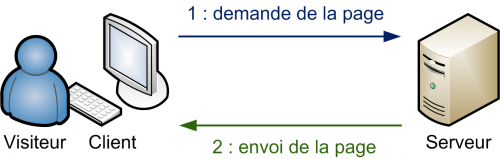
\includegraphics[width=.55\textwidth]{img/static.png}
\caption{Case of a static Html page}
\label{figure:static-page}
\end{figure}

\begin{figure}[!ht]
\centering
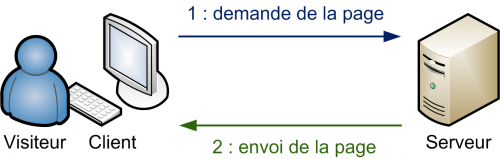
\includegraphics[width=.55\textwidth]{img/static.png}
\caption{Case of a dynamic page (for example a php page)}
\label{figure:dynamic-page}
\end{figure}

While the server will always deliver the same content for the same requested page, two different users might see two different things on their computer. 
The reason is that there are more than one web browser software application existing, and while they try to make it look the same, the process behind the display and interpretation of the content is not. Set aside Html content, which is quite processed in the same way among every browsers, issues arises with interpretation of
JavaScript and Stylsheets (CSS). For example, Firefox will understand the CSS property moz-border-radius while Google Chrome and Internet Explorer will not. 

Also, Firefox will not understand the JavaScript Object window.event while Google Chrome and Internet Explorer will. There are dozens of example like these ones.
While you can develop the server side part of the application in one language and not worry about its ability to always deliver the same content, you can't afford to develop the client side application for only one browser. This would result in many internet users not to be able to see the content as intended.

\begin{figure}[!ht]
\centering
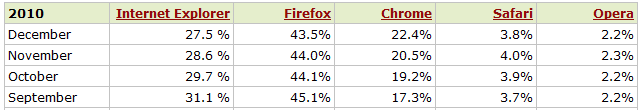
\includegraphics[width=.55\textwidth]{img/browser_statistics.png}
\caption{Market Share of Web Browser}
\label{figure:market-brosers}
\end{figure}

And as a web development company, that is even less of an option. (your clients won't like that if you tell them that only 30 of the internet users will be able to use their website.)
Web application that behaves the same way in multiple browser are called "cross-browser". 
My job was of course to make sure that every web content I created was cross-browser (at least for IE7, IE8, Chrome and FF).
At first, this can look like a hard task to accomplish, because you would need to be aware of each browser specificities. Fortunately, some tools exists to help you reach that goal.

\subsection{JavaScript}

JavaScript has some big differences between browsers. For example, to attach an event to an element, Firefox and Chrome uses the function addEventListener. Internet Explorer will not understand this function as it uses attachEvent for the same purpose. To see an example of how JavaScript can differ between browsers, refer to the Appendix B
Also, one of the purpose of JavaScript is being able to handle all the html elements in the web page to increase the user experience on the website. And again, there are some slight differences between every browser.

Because of all those disparities, people started to build APIs, which would considerably reduce the knowledge needed of those disparities to run a cross-browser JavaScript code. On of the most famous is jQuery. Simple, yet powerful, you can find in jQuery all the JavaScript functionalities, encapsulated in cross-browser functions. Ex: instead of having to test if the browser is IE to call the function attachEvent instead of addEventListener, you can just call the jQuery method bind to attach an event to an element. No need to learn the supported functions of each browser, you just need to learn a simple API. jQuery even simplifies some JavaScript functionalities, such as the use of Ajax.
%(cf piece of code w w/o jQuery).

\subsection{CSS}

Unlike in JavaScript, there is no API to help you with CSS (mainly because CSS is not a programming language). The huge issues in CSS arises when you want to make it work on Internet explorer (See Appendix \ref{annexe:JavaScript differences}). Usually, you are going to develop with Chrome or Firefox (Internet Explorer can be very slow so it can be frustrating to develop on it) where the same CSS is going to work on each other. It might even work in Internet Explorer 8 (with some really little adjustment on precise cases). But most of the time, you are going to have to do some adjustments so that it works on Internet Explorer 7. Those adjustment might be to just rethink the way of styling an element so that the same CSS will work on IE7 or completely tweaking the CSS just for Internet Explorer.

The last is called "CSS hacking". And fortunately, probably because Microsoft knows that his CSS handling is not that good, it introduced what is called conditional comments. It looks like a simple html comments in the html content, but IE knows it is aimed at him and can process it to add a specific Stylesheet. Other browsers will just ignore it, as it is a mere comment for them. (cg example html + speak about prefix * \_ etc.). 

\begin{figure}[!ht]
\centering
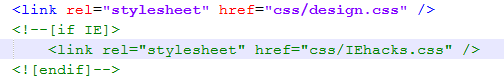
\includegraphics[width=.55\textwidth]{img/comments.png}
\caption{Conditional Comment}
\label{figure:conditional comment}
\end{figure}

Another way to tweak the CSS specifically for Internet Explorer is to add a specific prefix to each CSS property you want to be applied only to some Internet Explorer Versions. (prefix * : IE 7 and below,prefix \_: IE6 and below). The downside of this is that it renders the CSS invalid to the W3C specification.

Understanding all that, you can understand why creating a site builder application is even more of a challenge. Indeed, we have to provide the user that has no understanding of html, CSS or JavaScript the ability to create a cross-browser website. And that was an important point, because it could give us an advantage against other competitors, who are not always cross-browser compliant.
